\documentclass[10pt]{article}
\usepackage{tikz}
\usetikzlibrary{positioning,arrows}
\usetikzlibrary{shapes.geometric}
\renewcommand{\familydefault}{\ttdefault}
\tikzstyle{w}=[draw, circle, inner sep=8pt, minimum size=6pt, node distance=0.5cm, fill = lightgray]

\begin{document}
\begin{figure}[h]
	\centering
	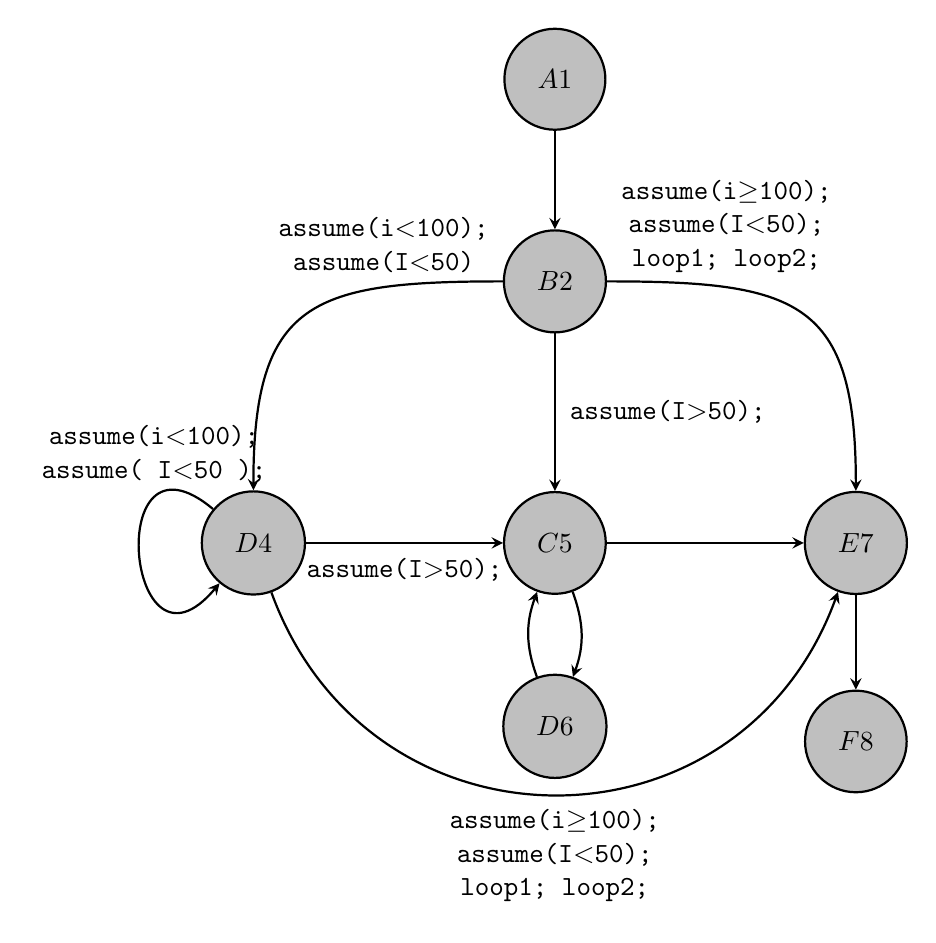
\begin{tikzpicture}[scale = 1,transform shape, -triangle 45, thick,
	el/.style = {inner sep = 5pt, align = center}]
	
	\node[w] (C5) at (0, 0) {$C5$};
 	\node[w] (D4) [left = 2.5cm of C5] {$D4$}; 
	\node[w] (D6) [below = 1cm of C5] {$D6$};
	\node[w] (B2) [above = 2cm of C5] {$B2$};
	\node[w] (E7) [right = 2.5cm of C5] {$E7$};
	\node[w] (F8) [below = 1.2cm of E7] {$F8$};
	\node[w] (A1) [above = 1.25cm of B2] {$A1$};

	\draw (D4) edge[->, >=stealth, in = -110, out = -70, looseness = 1.3] 
	node[el, below] {assume(i$\geq$100);\\assume(I$<$50);\\loop1; loop2;} (E7);
	
	\draw (B2) edge[->, >=stealth, in =   90, out = 180, looseness = 1.5, near start] 
	node[el, above] {assume(i$<$100);\\assume(I$<$50)} (D4);
	
	\draw (B2) edge[->, >=stealth, in =   90, out =   0, looseness = 1.5, near start]
	node[el, above] {assume(i$\geq$100);\\assume(I$<$50);\\loop1; loop2;} (E7);
	
	\draw (D4) edge[->, >=stealth, in = -130, out = 140, looseness =   5, near start]
	node[el, above] {assume(i$<$100);\\assume( I$<$50 );} (D4);
	
	\draw (C5) edge[->, >=stealth, in =   70, out = -70, looseness =   1] (D6);
	
	\draw (D6) edge[->, >=stealth, in = -110, out = 110, looseness =   1] (C5);
	
	\draw (B2) edge[->, >=stealth]
	node[el, right] {assume(I$>$50);} (C5);
	
	\draw (E7) edge[->, >=stealth] (F8);
	
	\draw (A1) edge[->, >=stealth] (B2);
	
	\draw (D4) edge[->, >=stealth] 
	node[el, below] {assume(I$>$50);} (C5);
	
	\draw (C5) edge[->, >=stealth] (E7);
	
	\end{tikzpicture}
  \label{fig:sat-reduction-edges}
\end{figure}
\end{document}
